\documentclass[a4paper, 12pt]{article}

%\usepackage{natbib}
\usepackage[english]{babel}
\usepackage{amsmath, amssymb}
\usepackage{parskip}
\usepackage{graphicx}
\usepackage{placeins}
\usepackage{url}

\DeclareMathOperator*{\argmax}{argmax}

\begin{document}

\title{AA2 Practical Assignment}
\author{Maarten de Jonge, Koen Keune, Edwin Odijk,\\ Francesco Stablum, Marysia Winkels}
\maketitle

\section*{Introduction}
%something something sampling based fitted Q-iteration/value-iteration, something something continuous
This report describes the extension on an old AA1 assignment for the AA2 course. The existing predator/prey game's environment was changed from discrete to continuous, and the game was optimized using sampling based fitted Q-iteration/value-iteration.%\cite{ng_lecture}\cite{musze}

FVI (Fitted Value Iteration) is an algorithm that is suited for
continuous state spaces with continuous features extracted from
the state. 
The value function of a certain state is inferred by
extracting at first the features $\phi(s^{(i)})$ 
after having sampled some states 
$s^{(1)}\ldots s^{(i)} \ldots s^{(m)}$, 
and then by fitting via linear regression
the respective estimated state values $y^{(i)}$ 
in order to obtain the vector
of weights $\theta$.

The estimated state values $y^{(i)}$ are calculated as follows:
for each action $a$ and state $s^{(i)}$, 
$k$ state transitions are performed by using probabilities from 
an MDP model.
An estimated $Q$-value for the $\langle a,s^{(i)}\rangle$ pair is obtained
by averaging the sums of rewards of $s^{(i)}$ and
discounted value of the
state obtained from the transition from $s^{(i)}$.
In this step the $V$-function from the previous iteration has been used,
which, at the first iteration, has been set to 0.

These estimated $Q$-values are then used in a Bellman-like 
backup operator which selects the highest $Q$-value across all actions,
and for the specific current $s^{(i)}$.
This will become the current estimated $V$-value for $s^{(i)}$. 
This value is denoted
by the symbol $y^{(i)}$ in order to highlight the fact that it's 
a quantity that is subject to regression.

Once all $y^{(\cdot)}$ values have been obtained,
the previously mentioned regression is performed.
This whole procedure is performed iteratively for a pre-determined
number of iterations.

\section*{Implementation} 
The algorithm has been implemented in one main function \texttt{fvi}
that resembles to a certain extent the pseudo-code
from Ng's lecture notes \cite{ng_lecture}.

Behavior has been parametrized by adding a number of lambda functions
as parameters to the function \texttt{fvi}:

\begin{itemize}
\item \texttt{sample\_states} is a function that returns the $s^{(1)}\ldots s^{(m)}$ sampled states
\item \texttt{sample\_actions} is a function that returns a set of sampled actions, which might be in principle sampled from a continuous distribution as well.
These action will then be used in order to calculate all $Q$-value
estimations for a certain state $s^{(i)}$.
\item \texttt{phi} is a function that will return a feature vector
$\phi(s^{(i)})$ for the state $s^{(i)}$ given as input.
A good feature vector representation is
crucial in order to obtain an acceptable regression.
\end{itemize}

The biggest change with regards to the discrete world previously implemented is
the action selection function. Rather than simply maximizing the value over a
small, finite set of actions, it now has to be maximized over an infinite
2-dimensional interval. Luckily, the value function is conveniently convex
(\ref{fig:V}) and can be optimized by means of gradient ascent or similar
methods.

\begin{figure}[h!]
  \centering
  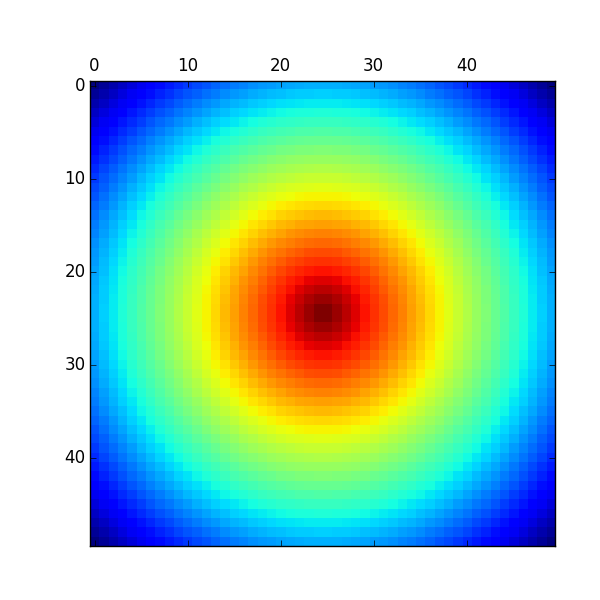
\includegraphics[width=0.5\textwidth]{V.png}
  \caption{A visual heatmap representation of the value function}
  \label{fig:V}
\end{figure}


We opted for a more brute-force method that makes use of the fact that
the $x$ and $y$ directions can be optimized separately: Given a state $s$, first
the optimal action in the $x$ direction is calculated as
\[
  x' = \argmax_x V(transition(s, [x, 0]))
\]
followed by the optimal action in the $y$ direction:
\[
  y' = \argmax_y V(transition(s, [x', y]))
\]

\paragraph{State transition function}
One notable difference from Ng's version is that in our implementation
the probabilistic model of state transition is not stated explicitly
as a definition of a probability of transitioning to a new state 
given a previous state and an action, but is replaced by
just using a state transition function, whose implementation
was much easier and intuitive.

\section*{Comparison of State Sampling Methods}
\FloatBarrier
We tested the influence of the state sampling method on the convergence rate of
the algorithm, where convergence is defined as the point where the current value
function in combination with our action selection results in an optimal policy.
The results can be found in figure \ref{fig:conv}. The x-axis shows number of
FVI iterations performed, while the y-axis shows the duration of the simulation
(i.e. the number of steps until the prey is caught) averaged over 100 runs. The
tested sampling methods were 11x11 grid sampling (sampling all the states of the
previous discrete world), 100 random samples, 10 random samples, and 1 random
samples. Random samples where resampled on each iteration of the algorithm.

\begin{figure}[htb]
  \centering
  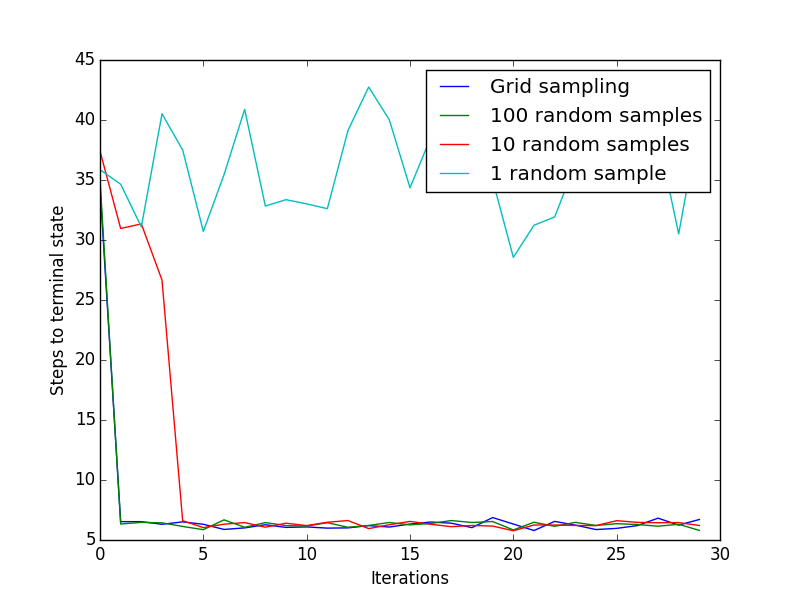
\includegraphics[width=0.8\textwidth]{convergence.png}
  \caption{Average simulation duration at each FVI iteration}
  \label{fig:conv}
\end{figure}

Although using only 1 sample takes a very long time to converge, the algorithm
can be seen to converge quite quickly for all other sampling methods, with 100
samples being slightly quicker than using only 10. This is further analyzed in
figure \ref{fig:n}, which plots the time to convergence as a function of the
number of random samples. These results were not averaged over multiple runs due
to time constraints. It shows that going from 1 to 2 samples gives a dramatic
increase in convergence speed, with a slow steady downwards curve afterwards.
The spike at 4 samples is likely a result of random factors.

\begin{figure}[htb]
  \centering
  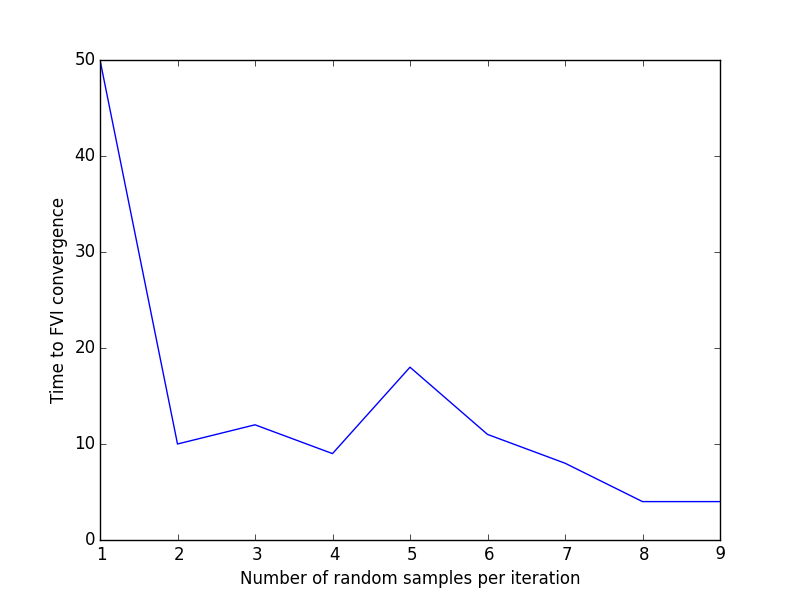
\includegraphics[width=0.8\textwidth]{n_samples.png}
  \caption{Time to convergence for various sampling densities}
  \label{fig:n}
\end{figure}

\FloatBarrier

\section*{Possible improvements}

Since the action space is continuous, different action sampling procedure
can be experimented. Moreover, different regressors for the 
$V$ function might be attempted,
such as \emph{Random Forests} or \emph{Support Vector Regression}.

The sampling of the states might also be focused on states that 
seem to be more probable, especially in the scenario of 
an online-focused variant
of \emph{FVI}. In the absence of such MDP probabilistic model,
easy-implementable techniques (with \texttt{sklearn}), such as
\emph{EM-Gaussian Mixture Models} can be fitted
after exploratory phases. Subsequently,
states might be sampled from the resulting \emph{GMM}.

\section*{Conclusion}
The FVI algorithm performs very well and converges upon the optimal policy
quickly. This is likely a result of the use of linear regression combined with
the nature of the MDP; the simple convex value function is well suited for being
linearly approximated. It retains this performance down to very low sampling
densities, with even just 2 random samples per iteration performing well.

\bibliographystyle{plain}
\bibliography{ref}

\end{document}
